\documentclass[a4paper]{article}

\usepackage[english]{babel}
\usepackage[utf8]{inputenc}
\usepackage{amsmath}
\usepackage{graphicx}
\usepackage{hyperref}
\usepackage[justification=centering]{caption} % Centré les captions des figures
\usepackage[colorinlistoftodos]{todonotes}

\title{SR03 - Projet 2 - Application Web Java EE - Plate-forme d'évaluation des compétences des stagiaires}

\author{Vallois Célestin - Mohamed Baaziz - Maxime Deranty}

\date{\today}

\begin{document}
\maketitle

\begin{abstract}

Le but de ce projet est avant tout de réaliser une application web en Java EE afin de s'initier à la programmation web côté serveur en réalisant une plate-forme en ligne d'évaluation des compétences des stagiaires via des QCM. Une liste de conditions et fonctionnalités nous est imposée, voici les grands lignes de chacune d'elles. (cf. énoncé pour une version détaillé)

\begin{itemize}

\item La plate-forme doit gérer dans un premier temps les utilisateurs selon s'ils sont administrateurs ou stagiaires.

\item L'administrateur peut créer et modifier des questionnaires avec les questions et réponses les composants.

\item La deuxième grande tâche de l'administrateur est de gérer les utilisateurs en les créant et modifiant. Remarque : lors de la création d'un utilisateur, un e-mail lui sera envoyé avec son mot de passe de plus de 6 caractères.

\item Les questionnaires sont composés de plusieurs questions eux même composé de plusieurs réponse mais seulement une réponse sera correcte par question.

\item Toutes les identités questionnaire, question, réponse et utilisateur possède un statut actif et inactif.

\item Finalement lors d'une évaluation d'un stagiaire, ce dernier effectue un "parcours" qui doit recenser son questionnaire, son score, le temps de passage et les réponses à chaque questions (On estime qu'un passage s'effectue sans pause).

\item L'aspect graphique n'a pas du tout été abordé durant ce sujet mais l'affichage visuel en pagination par exemple étant demandé si possible.

\end{itemize}

\end{abstract}

\section{Les choix technologiques}
\label{sec:introduction}

La première phase du projet fût le choix de nos futures technologies.

Comme demandé dans les objectifs de ce projet, nous avons utilisé \textbf{Java EE} (Java Enterprise Edition) afin d'effectuer ce projet en utilisant les \textit{servlets} et les \textit{JSP} pour créer dynamiquement les pages. Nous avons décider d'opter pour la dernière version, \textbf{Java 8} afin de ne pas nous priver des dernières fonctionnalités disponibles sur cette version, même si nous n'en avons pas forcément eu le besoin.
En complément de JEE, nous avons utilisé la \textbf{version 8 de Tomcat}, le fameux conteneur web libre de \textbf{servlets} et \textbf{JSP} (JavaServer Pages).

Enfin, nous devions utiliser une base de données, nous avons donc décider d'utiliser celle qui nous était fourni par l'UTC qui est une \textbf{base de données MySQL} sur le serveur \textit{tuxa.sme.utc} (il faut donc être connecté directement au réseau UTC pour y accéder ou bien posséder un VPN permettant de s'y connecter).

Petite remarque supplémentaire, nous avons eu besoin des bibliothèques suivante pour notre projet :
\begin{itemize}
\item \textbf{jstl-1.2.jar} pour l'utilisation des \textit{JSP} (JavaServer Pages) afin de créer nos pages web.
\item \textbf{mysql-connector-java-5.1.39-bin.jar} afin d'utiliser notre base de données MySQL.
\item \textbf{javax.mail.jax} afin d'utiliser l'\textbf{API JavaMail} pour l'envoie d'un e-mail lors de la création d'un compte.
\end{itemize}

Enfin, juste pour l'information, en terme d'IDE, nous utilisons \textbf{Eclipse Mars} afin de ne rencontrer aucuns problème avec le serveur Tomcat (problème survenu avec Eclise Indigo au début du projet). Mars(plus récent) semble donc plus robuste et portatif que son confrère plus agé. Le choix de l'IDE reste cependant libre selon les habitudes programmeurs.

Nous n'avons donc \textbf{pas utiliser de FrameWorks} afin de nous initier à JEE mais nous aurions très bien pu utiliser \textit{Spring} (comme vu en cours) avec même l'aide de l'application génératrice d'application web \textbf{JHipster} (l'application générée utilise alors AngularJS et le framework Spring).

\section{La structure du projet}
\label{sec:theory}

\subsection{Le mécanisme Java EE}

Afin de bien comprendre ce projet, il est important de cerner le fonctionnement d'une application JEE et son contenu

Un fichier \textbf{web.xml} comporte l'ensemble des "paths"(chemins/routes) attribués à une \textbf{servlet}. Cette dernière n'est rien d'autre qu'une classe Java de type servlet qui a pour but de créer dynamiquement des données au sein du serveur. Elle va effectué un traitement de la requête (en appelant la base de donnée MySQL dans notre projet si besoin ait par exemple) qu'elle reçoit afin d'envoyer une réponse (généralement sous forme de code HTML) au client. Il se peut alors que un fichier \textbf{JSP}. En effet le code générée par la servlet peut l'être \textit{à la volée} ou bien via l'exécution d'un autre fichier Java comme par exemple un fichier JSP.

Elle possède aussi des fichiers stockés dans le dossier \textbf{WEB-INF} qui sont dit publics car ils sont accessibles sans servlets (au contraire des pages JSP précédentes). Dans le cas de notre projet, il n'y aura que le fichier \textit{web.xml} (qui est donc accessible au public) et nos librairies. Si nous avions voulu soigner l'esthétique, les fichiers CSS, JavaScripts et autres fichiers multimédia pouvant être accessible de tous alors dû s'y trouver.

\subsection{L'organisation de la plate-forme d'évaluation}

Pour ce projet nous avons essayé de respecter au le modèle \textbf{MVC}, nous avons donc l'organisation suivantes de nos fichiers sources présent dans \textit{src} : 

\begin{itemize}

\item \textbf{beans} pour la partie \textit{modèle}. Il regroupe toutes les classes métiers. Chaque entité présente dans notre modèle UML du projet (cf \ref{sql_model}) possède sa classe métier. On pourra noter que chacune de ces classes possède aussi sa table dans notre base MySQL. Comme il s'agit de représentant de notre table, chaque classe possède les attributs indiqué dans notre modèle et table, les méthodes sont des accesseurs et modificateurs (get/set) et constructeurs.

\item \textbf{controllers} pour un bout de la partie \textit{contrôle}. Il rassemble les servlets qui traitent les requêtes HTTP.
\item \textbf{dao}, deuxième partie pour le \textit{contrôle}. Ces classes java servent à la gestion de la base de données MySQL. Cela peut être pour des recherches, des ajouts ou des modifications dans cette base.
\item \textbf{utils} regroupe les fonctions \textit{utilitaire} de Java comme son nom l'indique afin d'éviter la redondance de code.

\end{itemize}

La partie \textit{Vue} qui n'a pas été abordé dans les précédents fichiers est composée des fichiers JSP qui affiche les pages HTML retourner au navigateur par la servlet si elle ne génère par sa page à la volée. Ses JSP sont présents dans la partie \textit{WebContent} du projet. C'est dans cette partie que ce trouve \textit{WEB-INF} évoqué précédemment avec les bibliothèques utilisé, web.xml et nos pages JSP.

Maintenant que nous avons vu l'organisation du projet, nous allons aborder notre modélisation de notre base de données MySQL (cf. \ref{fig:model_uml}).

\subsection{Le modèle du projet}
\label{sql_model}

% TO BE UPDATED
\begin{figure}[h]
\centering
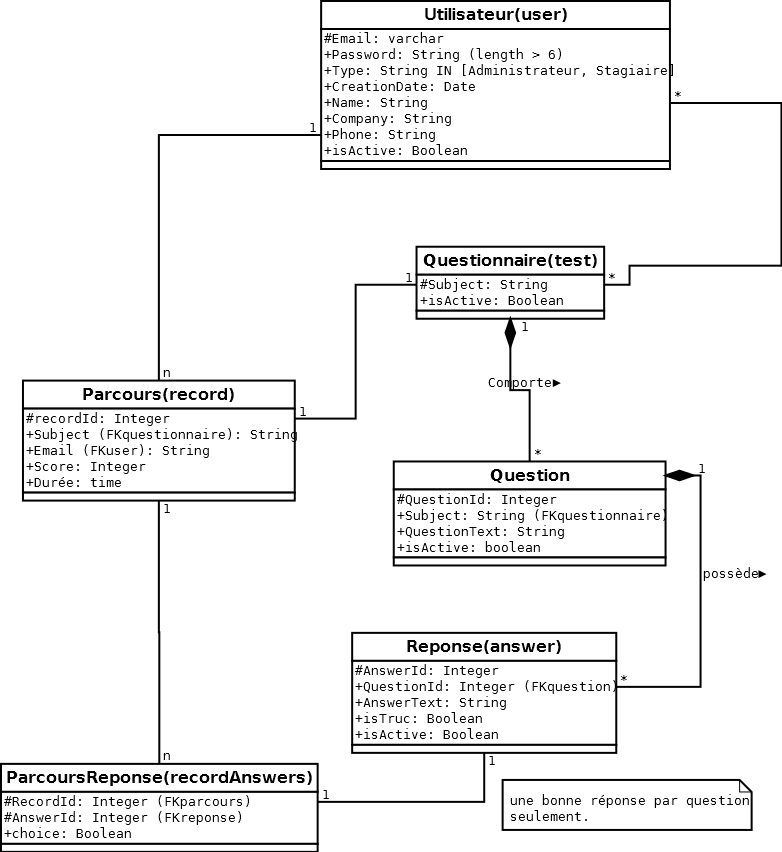
\includegraphics[width=1\textwidth]{Modele.png}
\caption{\label{fig:model_uml}Modèle UML de notre Base de donnée MySQL}
\end{figure}

La création de ce modèle a été la première étape de notre projet (avant même le choix des technologies). Nous l'avons utilisé afin de créer nos tables dans notre base de données mais aussi nos classes-métiers au sein du répertoires \textit{beans}.
On pourra remarquer qu'il n'est pas en 3NF ($3^{eme}$ forme normale), il aurait fallut par exemple alors créer une table \textbf{entreprise} afin d'éviter les redondances etc... Mais là n'était pas le but de ce projet. Il est donc ici pour présenter les liens entre les différentes tables. 

Nous avons voulus simplifier ce projet. Cependant nous aurions pu largement améliorer ce modèle pour le rendre plus robuste en intégrant des clé artificielles qui \textit{s'auto-incrémente} (sauf pour l'email), des dates créer automatiquement avec \textit{CURRENT-TIMESTAMP} afin de garder un historique des dernières modifications. 

De nombreuses conditions réalisées sur la table ne sont pas indiqués sur ce modèle comme les champs \textit{NOT NULL}, \textit{UNIQUE} et les \textit{CHECK}(vérification d'existence d'une condition comme la taille minimale de 6 caractères du mot de passe) sur d'autres. Ces conditions sont très simples à deviner à partir du sujet et dû à la petite taille du modèle qui est normalement très facilement compréhensible au premier coup d'œil.

Il est possible d'aller beaucoup plus loin dans la gestion des bases de données avec les \textit{triggers} d'événement par exemple. Ils permettent d'effectuer certaines actions ou vérifications supplémentaires lors de changement sur la base de données (la personne qui modifie le questionnaire est-elle bien un administrateur etc...) Nous n'avons pas été jusque là mais cela n'est pas à oublier si jamais l'on souhaite développer plus en profondeur ce projet.

\section{Les fonctionnalités du projet}

\subsection{La Gestion des Utilisateurs}

Les utilisateurs sont regroupés 2 groupes : d'abord les administrateurs puis les stagiaires. 
Les administrateurs peuvent créer, modifier et supprimer n’importe quelle information de tous les utilisateurs qui sont regroupé au sein d'une pagination. Ils vont être les grands partisans de la gestion des utilisateurs
Les stagiaires ne peuvent quant à eux que modifier des informations sur leur compte.
Lors de la création d’un nouvel utilisateur. Cette-dernière va déclencher l’envoie d’un mail contenant l'identifiant (l'adresse mail) et le mot de passe de la personne. 
% CE QUON A PAS FAIT
Nous n'avons pas réalisé la partie modification d'un utilisateur au sein d'une connexion en tant que stagiaire car il s'agissait de la même implémentation que pour la partie modification des utilisateur sauf qu'il ne concernait que lui-même.

\subsection{La Gestion des questionnaires}

Les questionnaires sont intégralement gérés par les administrateurs. Les stagiaire n'ont une nouvelle fois aucun pouvoir sur leur gestion.
Les administrateurs peuvent créer, modifier ou même supprimer un questionnaire. 
La création d’un questionnaire se fait avec un nom et un sujet.  
Ensuite vient la partie question et réponse. Pour chaque questionnaire, l'administrateur peut créer, modifier et supprimer les questions et réponses associées à ce questionnaire. Il peut aussi modifier l'ordre des questions.

% CE QUON A PAS FAIT 

\subsection{La Gestion des parcours}

La dernière partie concerne les parcours. Les stagiaires peuvent effectuées ses parcours et observer leur score sur ces derniers. Ces parcours possède le score et le temps de passage du questionnaire, ainsi que les réponses qu'il a mis.

% CE QUON A PAS FAIT

\subsection{Remarques}

% Si vous avez des remarques
%Sur ce projet nous avons/n'avons pas ...

\section{Conclusion}

\subsection{Les difficultés rencontrées}

Durant ce projet, beaucoup de fonctionnalités étaient redondantes et le temps nous a manqué.
Être $3$ n'était pas forcément aisé pour gérer les parties de chacun.

Il nous a fallut apprendre le Java EE dans un premier temps, nous remettre à la gestion de base de données MySQL afin d'avancer ce projet.

Avec plus de temps, beaucoup de points auraient pu être développé, améliorer comme par exemple la gestion des personnes connectés afin de vérifier qu'il s'agisse bien en permanence d'un administrateur/stagiaire via un filtre de connexion.

\subsection{Conclusion}

En conclusion ce projet nous aura permis de nous initier à Java EE, afin de découvrir cette technologie que nous n'avions pas utiliser avec l'utilisation des pages JSP et des servlets principalement. Nous avons dû mettre un place un modèle MVC et gérer notre base de données MySQL.
Même si toutes les fonctionnalités n'ont pas pu être réalisées, il nous aura permis de bien appréhender Java EE et la création d'une application web.
En résumé, il nous aura permis de voir la programmation côté-serveur avant le prochain projet qui sera un web-service. Finalement, il nous aura permis de mettre en pratique la théorie étudiée en cours à l'aide d'un projet très instructif et complet.

% Mettre des images de l'appli en annexe !
\newpage
\section{Annexes}

% \begin{figure}[h]
% \centering
% 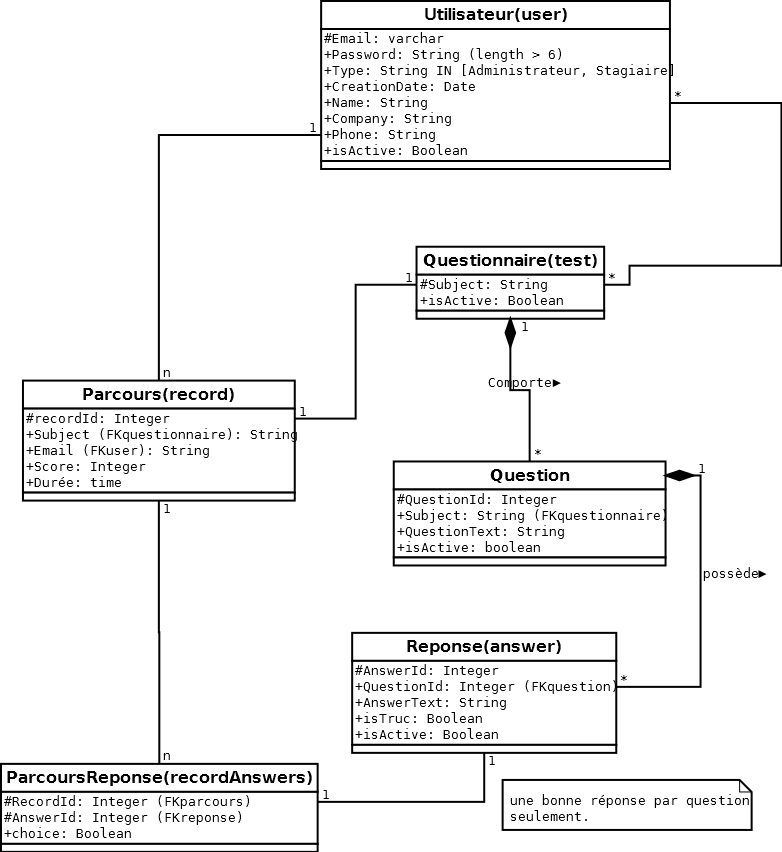
\includegraphics[width=1\textwidth]{Modele.png}
% \caption{\label{fig:model_uml}Modèle UML de notre Base de donnée MySQL}
% \end{figure}

\end{document}